%-------------------------------------------------------
% SLEPc Users Manual
%-------------------------------------------------------
\chapter{\label{cap:int}Introduction}
%-------------------------------------------------------

\noindent \slepc, the {\em Scalable Library for Eigenvalue Problem Computations}, is a software package for the solution of large sparse eigenvalue problems on parallel computers. 

	Together with linear systems of equations, eigenvalue problems are a very important class of linear algebra problems. The need for the numerical solution of these problems arises in many situations in science and engineering. There is a strong demand for solving  problems associated with stability and vibrational analysis in practical applications, which are usually formulated as large sparse eigenproblems.

	Computing eigenvalues is essentially more difficult than solving linear systems of equations. This has resulted in a very active research activity in the area of computational methods for eigenvalue problems in the last years, with many remarkable achievements. 
	However, these state-of-the-art methods and algorithms are not easily transferred to the scientific community, and, apart from a few exceptions, scientists keep on using traditional well-established techniques.
	
	The reasons for this situation are manifold. First, new methods are increasingly complex and difficult to implement and therefore robust implementations must be provided by computational specialists, for example as software libraries. The development of such libraries requires to invest a lot of effort but sometimes they do not reach normal users due to a lack of awareness.
	
	In the case of eigenproblems, using libraries is not straightforward. It is usually recommended that the user understands how the underlying algorithm works and typically the problem is successfully solved only after several cycles of testing and parameter tuning. Methods are often specific for a certain class of eigenproblems (e.g. complex symmetric) and this leads to an explosion of available algorithms from which the user has to choose. Not all these algorithms are available in the form of software libraries, even less frequently with parallel capabilities.
	
	A further obstacle appears when these methods have to be applied in a large software project developed by inter-disciplinary teams. In this scenery, libraries must be able to interoperate with already existing software and with other libraries, possibly written in a different programming language. In order to cope with the complexity associated with such large software projects, libraries must be designed carefully in order to overcome hurdles such as different storage formats. In the case of parallel software, care must be taken also to achieve portability to a wide range of platforms with good performance and still retain flexibility and usability. 

	The \slepc library is an attempt to address this complexity and provides a set of tools that can be used to obtain a solution in many applications. \slepc is based on \petsc, the Portable, Extensible Toolkit for Scientific Computation \citep{Balay:2002:PUM}, and, therefore, a large percentage of the complexity is avoided since \slepc relies on \petsc\ for all low level implementation details. \slepc focuses on high level features structured around a few types of objects. It offers a growing number of solution methods as well as interfaces to integrate well-established eigenvalue packages such as \arpack.

%---------------------------------------------------
\section{Getting Started}

	\slepc is a general library for the solution of eigenvalue problems, in the sense that it covers standard and generalized eigenvalue problems, both Hermitian and non-Hermitian, with either real or complex arithmetic. This manual assumes that the reader is familiar with eigenvalue problems, their basic mathematical properties and the basic techniques and methods to solve them. A brief introduction to the topic is included in section \ref{sec:eig}. A nice introduction of eigenvalue problems and an overview of methods can be found in \citep{Golub:2000:EC2}.
	
	The emphasis of \slepc is on methods and techniques appropriate for problems in which the associated matrices are sparse, for example, those arising after the discretisation of partial differential equations. Therefore, most of the methods offered by the library are projection methods or other methods with similar properties. Examples of these methods are Arnoldi, Lanczos and Subspace Iteration, to name a few. A comprehensive description of state-of-the-art methods of this kind can be found in \citep{Bai:2000:TSA}. \slepc contains implementations of the basic methods as well as a growing number of more sophisticated algorithms.

	The Portable, Extensible Toolkit for Scientific Computation (\petsc) uses modern programming paradigms to ease the development of large-scale scientific application codes in Fortran, C, and C++ and provides a powerful set of tools for the numerical solution of partial differential equations and related problems on high-performance computers. \slepc is based on \petsc, and this means that \petsc\ must be previously installed in order to use \slepc. \petsc\ users will find \slepc very easy to use, since it enforces the same programming paradigm. Those readers which are not acquainted with \petsc\ are highly recommended to familiarize with it before proceeding with \slepc. An introduction to \petsc\ is included in section \ref{sec:petsc}.

	\slepc can be considered an extension of \petsc\ providing all the functionality necessary for the solution of eigenvalue problems. Figure \ref{fig:slepc} shows a diagram of all the different objects included in \petsc\ (on the left) and those added by \slepc (on the right). \petsc\ is a prerequisite for \slepc and users should be familiar with basic concepts such as vectors and matrices in order to use \slepc. Therefore, together with this manual we recommend to use the \petsc\ Users Manual \citep{Balay:2002:PUM}.

\begin{figure}[t]
\centering
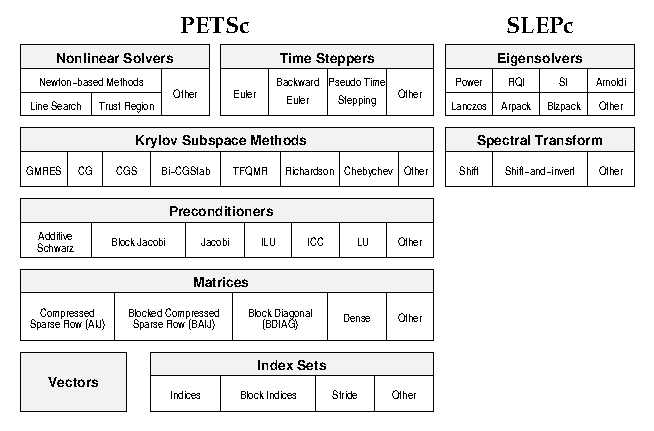
\includegraphics[width=12cm]{slepc-fig.eps}
\caption{\label{fig:slepc}Numerical components of \petsc\ and \slepc.}
\end{figure}

The complete \slepc distribution, users manual, manual pages, and additional information are available via the \slepc home page at 
	\begin{quote}
	\begin{center}
	\url{\slepchome}.
	\end{center}
	\end{quote}
The \slepc home page also contains details regarding installation, new features and changes in recent versions of \slepc, and more information.

Within the \slepc distribution, the directory 
\Verb!${SLEPC_DIR}/docs!
%\texttt{\$\{SLEPC\_DIR\}/docs}
 contains all the documentation of the library. Manual pages for all \slepc functions can be accessed on-line at \url{\slepchome/document.htm}. These manual pages provide hyperlinked indices (organized by both concepts and routine names) to the source code and enable easy movement among related topics.  The file \texttt{slepc.ps} contains the Postscript form of the \slepc Users Manual (this document). A PDF version is also available.

\medskip
\textbf{Note to Fortran Programmers}: As in the case of \petsc, in this manual  all the examples and calling sequences are given for the C/C++ programming languages. However, Fortran programmers can use most of the functionality of \slepc and \petsc\ from Fortran, with only minor differences in the user interface. Section \ref{sec:fortran} provides a discussion of the differences between using \slepc from Fortran and C, as well as complete Fortran examples. 

%---------------------------------------------------
\section{Installation}
\label{sec:inst}

	This section gives an overview of the installation procedure. For full installation instructions see \url{\slepchome/install.htm}.

	Previously to the installation of \slepc, the system must have an appropriate version of \petsc\ installed. Table \ref{tab:ver} shows a list of \slepc versions and their corresponding \petsc\ versions. \slepc versions marked as major releases are those which incorporate some new functionality. The rest are just adaptations required for a new \petsc\ release and may also include bug fixes.

\begin{table}[ht]
\centering
\begin{tabular}{ccccc}
\slepc version &     \petsc versions &  Major  & Release date \\ \hline
         2.1.0 &               2.1.0 & $\star$ & Not released \\
         2.1.1 & 2.1.1, 2.1.2, 2.1.3 &         & Dec 2002     \\ 
         2.1.5 &        2.1.5, 2.1.6 &         & May 2003     \\ 
         2.2.0 &               2.2.0 & $\star$ & Apr 2004     \\
 \slepcversion &       \slepcversion & $\star$ & Aug 2004     \\ \hline
\end{tabular}
\caption{\label{tab:ver} Correspondence between \slepc and \petsc\ releases.}
\end{table}

	There are two possible ways of installing \petsc: automatically (with configure scripts) or manually. \slepc does not support automatic installation yet. For a manual installation of \petsc, the user simply sets the environment variables \ident{PETSC\_DIR} and \ident{PETSC\_ARCH} and types \texttt{make}. Apart of this, some customization may be necessary, see the \petsc\ documentation for details.

	The installation process for \slepc is very similar. The main steps are described next. Note that prior to this steps, optional packages must have been installed. If any of these packages is installed afterwards, recompilation is necessary. Refer to \url{\slepchome/install.htm} or to section \ref{sec:wrap} for details about installation of some of these packages.

\begin{enumerate}
	\item Unbundle the distribution file \Verb!slepc.tgz! with a usual command such as \Verb!gunzip -c slepc.tgz | tar xvf -!. This will create a directory and unpack the software there.
	\item Refer to \url{\slepchome/download.htm} for available patches to the latest \slepc release.
	\item Set the environment variable \ident{SLEPC\_DIR} to the full path of the \slepc home directory, for example,
	\begin{Verbatim}[fontsize=\small]
	setenv SLEPC_DIR /home/username/slepc-2.2.x
	\end{Verbatim}
	In addition to this variable, \ident{PETSC\_DIR} and \ident{PETSC\_ARCH} must also be set correctly, the first one pointing to the \petsc\ home directory and the other containing the selected architecture.% (remember that \petsc\ allows several versions compiled for different architectures to coexist in the same directory tree).
	\item Edit the file \Verb!${SLEPC_DIR}/bmake/${PETSC_ARCH}/packages! to indicate the local installation of optional software packages such as \arpack. If there exists no directory named \Verb!bmake/${PETSC_ARCH}! for the value of \Verb!${PETSC_ARCH}! you are using, then create it similar to the existing ones.
	\item In the \slepc home directory, type
	\begin{Verbatim}[fontsize=\small]
	make BOPT=g
	\end{Verbatim}
      to build a debugging version of \slepc, or
	\begin{Verbatim}[fontsize=\small]
	make BOPT=O
	\end{Verbatim}
      to build an optimized version of the \slepc libraries. The flag \ident{BOPT} determines what type of libraries are built (i.e., specifies compiler options). Other available alternatives are \Verb!BOPT=[g_complex,O_complex]! for complex numbers versions (see section \ref{sec:complex}).
	\item If the installation went smoothly, then try running some test examples with the command
	\begin{Verbatim}[fontsize=\small]
	make BOPT=g slepc_testexamples >& examples_log 
	\end{Verbatim}
     Examine the file \Verb!examples_log! for any obvious errors or problems.
	\item The Fortran libraries are built automatically during the installation outlined above. To compile and test the Fortran examples, use the command
	\begin{Verbatim}[fontsize=\small]
	make BOPT=g slepc_testfortran >& fortran_log
	\end{Verbatim}
\end{enumerate}
	
%	For details about availability of \slepc on Windows platforms, see the up-to-date information in \url{\slepchome/install.htm}.
%---------------------------------------------------
\section{Running \slepc Programs}

Before using \slepc, the user must first set the environment variable
\ident{SLEPC\_DIR}, indicating the full path of the directory in which \slepc has been installed. For example, under the UNIX C shell a command of the form
	\begin{Verbatim}[fontsize=\small]
	setenv SLEPC_DIR /software/slepc
	\end{Verbatim}
can be placed in the user's \Verb!.cshrc! file. 
In addition, the user must set the two environment
variables required by \petsc, that is, \ident{PETSC\_DIR}, to indicate the full path of the \petsc\ installation, and \ident{PETSC\_ARCH} to specify the architecture (e.g., \texttt{rs6000},
\texttt{solaris}, \texttt{IRIX}, etc.)  on which \petsc\ is being used.  The utility
 \Verb!${PETSC_DIR}/bin/petscarch! can be used for this purpose.  For example,
	\begin{Verbatim}[fontsize=\small]
	setenv PETSC_ARCH `$PETSC_DIR/bin/petscarch`
	\end{Verbatim}
can be placed in a \Verb!.cshrc! file.  Thus, even if several machines of different
types share the same filesystem, \ident{PETSC\_ARCH} will be set correctly
when logging into any of them. 

All \petsc\ programs use the MPI (Message Passing Interface) standard
for message-passing communication \citep{MPI-Forum:1994:MMI}.  Thus, to execute
\slepc programs, users must know the procedure for launching MPI jobs
on their selected computer system(s).  For instance, when using the
\mpich\ implementation of MPI and many others, the \texttt{mpirun} command can be used to initiate a program as in the following example that uses eight processors:
	\begin{Verbatim}[fontsize=\small]
	mpirun -np 8 slepc_program [arguments]
	\end{Verbatim}

All \petsc-compliant programs support the use of the \Verb!-h!
or \Verb!-help! option as well as the \Verb!-v! or \Verb!-version! option. In the case of \slepc programs, specific information for \slepc is also displayed.

%---------------------------------------------------
\section{Writing \slepc Programs}

Most \slepc programs begin with a call to \rutina{SlepcInitialize}
	\begin{Verbatim}[fontsize=\small]
	SlepcInitialize(int *argc,char ***argv,char *file,char *help);
	\end{Verbatim}
which initializes \slepc, \petsc\ and MPI. This subroutine is very similar to \rutina{PetscInitialize}, and the arguments have the same meaning. In fact, internally \rutina{SlepcInitialize} calls \rutina{PetscInitialize}.
In Fortran the initialization command has the form
	\begin{Verbatim}[fontsize=\small]
	SlepcInitialize(character file,integer ierr)
	\end{Verbatim}

After this initialization, \slepc programs can use communicators defined by \petsc. In most cases users can employ the communicator \ident{PETSC\_COMM\_WORLD} to indicate all processes in a given run and \ident{PETSC\_COMM\_SELF} to indicate a single process. MPI provides routines for generating new communicators consisting of subsets of processors, though most users rarely need to use these. \slepc users need not program much message passing directly
with MPI, but they must be familiar with the basic concepts of message
passing and distributed memory computing.

All \slepc routines return an integer indicating whether an error has
occurred during the call.  The error code is set to be nonzero if an
error has been detected; otherwise, it is zero.  For the C/C++
interface, the error variable is the routine's return value, while for
the Fortran version, each \slepc routine has as its final argument an
integer error variable. 

All \slepc programs should call \rutina{SlepcFinalize}
as their final (or nearly final) statement, as given below in the C/C++
and Fortran formats, respectively:
	\begin{Verbatim}[fontsize=\small]
	ierr = SlepcFinalize();
	call SlepcFinalize(ierr)
	\end{Verbatim}
This routine handles options to be called at the conclusion of
the program, and calls \rutina{PetscFinalize}
if \rutina{SlepcInitialize}
began \petsc.


%---------------------------------------------------
\section{Simple \slepc Example}
\label{sec:simpleex}

To help the user start using \slepc immediately, a simple example is listed next which solves an eigenvalue problem associated with the
one-dimensional Laplacian operator discretized with finite differences.  This
example can be found in \Verb!${SLEPC_DIR}/src/examples/ex1.c!.
Following the code we highlight a few of the most important parts of this example.  

\MyVerbatimInput{${SLEPC_DIR}/src/examples/ex1.c}

\subsubsection*{Include Files}

The C/C++ include files for \slepc should be used via statements such as
	\begin{Verbatim}[fontsize=\small]
	#include "slepceps.h"
	\end{Verbatim}
where \Verb!slepceps.h! is the include file for the \ident{EPS} component.
Each \slepc program must specify an
include file that corresponds to the highest level \slepc objects
needed within the program; all of the required lower level include
files are automatically included within the higher level files. 
For
example, \Verb!slepceps.h! includes \Verb!slepcst.h! (spectral transformations),
and \Verb!slepc.h! (base \slepc file).  
The \slepc include files are located in the directory 
\Verb!${SLEPC_DIR}/include!.

\subsubsection*{The Options Database}

All the \petsc\ functionality related to the options database is available in \slepc. This allows the user to input control data
at run time very easily. In this example the command
\Verb!PetscOptionsGetInt(PETSC_NULL,"-n",&n,PETSC_NULL);! checks whether the user has
provided a command line option to set the value of \Verb!n!, the
problem dimension.  If so, the variable \Verb!n! is set accordingly;
otherwise, \Verb!n! remains unchanged.

\subsubsection*{Vectors and Matrices}

Usage of matrices and vectors in \slepc is exactly the same as in \petsc.
The user can create a new parallel or sequential matrix, \texttt{A}, which
has \texttt{M} global rows and \texttt{N} global columns, with the routine
\rutina{MatCreate}
	\begin{Verbatim}[fontsize=\small]
	MatCreate(MPI_Comm comm,int m,int n,int M,int N,Mat *A);
	\end{Verbatim}
where the matrix format can be specified at runtime. The example creates a matrix, sets the nonzero values with \rutina{MatSetValues} and then assembles it.

\subsubsection*{Eigensolvers}

Usage of eigensolvers is very similar to other kinds of solvers provided by \petsc.
After creating the matrix (or matrices) that define the problem,
$Ax = kx$ (or $Ax=kBx$), the user can then use \ident{EPS} to solve the system 
with the following sequence of commands: 
\findex{EPSCreate} \findex{EPSSetOperators}
\findex{EPSSetFromOptions} \findex{EPSSolve} \findex{EPSDestroy}
	\begin{Verbatim}[fontsize=\small,numbers=none]
	EPSCreate(MPI_Comm comm,EPS *eps);
	EPSSetOperators(EPS eps,Mat A,Mat B);
        EPSSetProblemType(EPS eps,EPSProblemType type);
	EPSSetFromOptions(EPS eps);
	EPSSolve(EPS eps);
	EPSGetIterationNumber(EPS eps,int *its);
	EPSGetConverged(EPS eps, int *nconv);
	EPSGetEigenpair(EPS eps,int i,PetscScalar *kr,PetscScalar *ki,
               Vec xr,Vec xi);
	EPSDestroy(EPS eps);
	\end{Verbatim}
The user first creates the \ident{EPS} context and sets the operators
associated with the eigensystem as well as the problem type. The user then sets various options for
customized solution, solves the problem, retrieves the solution, 
and finally destroys the \ident{EPS} context.
Chapter~\ref{cap:eps} describes in detail the \ident{EPS} package, including
the options database which enables the user to customize the solution
process at runtime by selecting the solution algorithm and also specifying the convergence tolerance, setting various monitoring routines, etc.

\subsubsection*{Spectral Transformation}

In the example program above there is no explicit reference to spectral transformations. However, an \ident{ST} object is handled internally so that the user is able to request different transformations such as shift-and-invert.
Chapter~\ref{cap:st} describes the \ident{ST} package in detail.

\subsubsection*{Error Checking}

All \slepc routines return an integer indicating whether an error
has occurred during the call.  The \petsc\ macro \Verb!CHKERRQ(ierr)!
checks the value of \Verb!ierr! and calls the \petsc\ error handler
upon error detection.  \Verb!CHKERRQ(ierr)! should be used in all
subroutines to enable a complete error traceback. See the \petsc\ manual 
for full details.

\subsubsection*{Writing Application Codes with \slepc}

The examples provided in the \Verb!src/examples! directory demonstrate the software usage
and can serve as templates for developing
custom applications.
To write a new application program using \slepc, we suggest the
following procedure:
\begin{enumerate}
\item Install and test \slepc according to the instructions at the \slepc web site.
\item Copy the \slepc example 
      that corresponds to the class of problem of interest (e.g.,
      singular value decomposition).
\item Copy the makefile within the example directory
      (or create a new one as explained in section \ref{sec:makefile});
      compile and run the example program.
\item Use the example program as a starting point for developing a custom code.
\end{enumerate}


%---------------------------------------------------
\section{Directory Structure}

	The directory structure of the \slepc software is very similar to that in \petsc. The root directory of \slepc contains the following directories:
\begin{description}
\item[\texttt{bmake}] - Base \slepc makefile directory. Includes subdirectories for various architectures.
\item[\texttt{docs}] - All documentation for \slepc, including this manual. The subdirectory \texttt{manualpages} contains the on-line manual pages of each \slepc routine.
\item[\texttt{include}] - All include files for \slepc that are visible to the user.
\item[\texttt{include/finclude}] - \slepc include files for Fortran programmers using the .F suffix.
\item[\texttt{lib}] - Location of all the generated libraries for each combination of \texttt{BOPT} and architecture.
\item[\texttt{src}] - The source code for all \slepc components, which currently includes
\begin{description}
\item \texttt{sys} - general system-related routines.
\item \texttt{eps} - eigenvalue problem solver.
\item \texttt{st} - spectral transformation.
\item \texttt{fortran} - Fortran interface stubs.
\item \texttt{examples} - example programs.
\item \texttt{mat/examples} - matrices used by some examples.
\end{description}
\end{description}

Each \slepc source code component directory has the following subdirectories:
\begin{description}
\item \texttt{interface} - The calling sequences for the abstract interface to the components. Code here does not know about particular implementations.
\item \texttt{impls} - Source code for one or more implementations.
\end{description}

